\def\thoigian{90}%--Thời gian
\de{Đề số 3}{Chương I. Mệnh đề và Tập hợp}
\everymath{\color{blue}}
\begin{center}
	\textbf{PHẦN 1 - Câu trắc nghiệm nhiều phương án lựa chọn.}
\end{center}
\setcounter{ex}{0}
%============Câu 1=======================
\begin{ex}%[0D1N1-1]%[KNTT - Lớp 10 - Nguyễn Thanh Phong]
Phát biểu nào là mệnh đề chứa biến?
\choice
{$\pi^2 \approx 10$}
{$2 < \pi$}
{\True $x + 2y = 5$}
{Hà Nội là thủ đô của Việt Nam}
\loigiai{
Ta thấy $x+2y=5$ là mệnh đề chứa biến.
}
\end{ex}
%============Câu 50======================
\begin{ex}%[0D1H4-3]%[Dự án A-Đợt 10 HKII NH24-25-Nguyễn Thanh Phong]
	Trong các mệnh đề sau, mệnh đề nào có mệnh đề đảo đúng?
\choice
{\lq\lq Nếu $a>b$ thì $a^2>b^2$\rq\rq}
{\True \lq\lq Nếu tích $ab$ của hai số nguyên $a$ và $b$ là một số lẻ thì $a$, $b$ là các số lẻ \rq\rq}
{\lq\lq Nếu một tứ giác là hình thoi thì có hai đường chéo vuông góc với nhau\rq\rq}
{\lq\lq Nếu một số nguyên chia hết cho $6$ thì nó chia hết cho $3$\rq\rq}
\loigiai{
Mệnh đề có mệnh để đảo \textbf{đúng} là \lq\lq Nếu tích $ab$ của hai số nguyên $a$ và $b$ là một số lẻ thì $a$, $b$ là các số lẻ\rq\rq. \\
Ta có mệnh đề đảo của mệnh đề trên là \lq\lq Nếu $a$, $b$ là các số lẻ thì tích $ab$ của hai số nguyên $a$ và $b$ là một số lẻ\rq\rq. 
}
\end{ex}
%============Câu 4=======================
\begin{ex}%[0D1N1-5]%[KNTT - Lớp 10 - Nguyễn Thanh Phong]
Phủ định của mệnh đề \lq\lq$\forall x \in \mathbb{R}$, $x^2 - 4x < 0$\rq\rq \,là mệnh đề:
\choice
{\True $\exists x \in \mathbb{R}$, $x^2 - 4x \geq 0$}
{$\forall x \in \mathbb{R}$, $x^2 - 4x \geq 0$}
{$\exists x \in \mathbb{R}$, $x^2 - 4x < 0$}
{$\exists x \in \mathbb{R}$, $x^2 - 4x > 0$}
\loigiai{
    Phủ định của mệnh đề \lq\lq$\forall x \in \mathbb{R}$, $x^2 - 4x < 0$\rq\rq \,là $\exists x \in \mathbb{R},\, x^2 - 4x \geq 0$.
}
\end{ex}
%============Câu 12======================
\begin{ex}%[0D1H4-1]%[Dự án A-Đợt 10 HKII NH24-25-Nguyễn Thanh Phong]
	Trong các mệnh đề sau, mệnh đề nào có mệnh đề đảo đúng?
\choice
{Nếu tứ giác $ABCD$ là hình chữ nhật thì tứ giác $ABCD$ có hai đường chéo bằng nhau}
{Nếu số nguyên $n$ có chữ số tận cùng là $5$ thì số nguyên $n$ chia hết cho $5$}
{\True Nếu tứ giác $ABCD$ có hai đường chéo cắt nhau tại trung điểm mỗi đường thì tứ giác $ABCD$ là hình bình hành}
{Nếu tứ giác $ABCD$ là hình thoi thì tứ giác $ABCD$ có hai đường chéo vuông góc với nhau}
\loigiai{
Mệnh đề có mệnh để đảo \textbf{đúng} là \lq\lq Nếu tứ giác $ABCD$ có hai đường chéo cắt nhau tại trung điểm mỗi đường thì tứ giác $ABCD$ là hình bình hành\rq\rq. \\
Ta có mệnh đề đảo của mệnh đề trên là \lq\lq Nếu tứ giác $ABCD$ là hình bình hành thì tứ giác $ABCD$ có hai đường chéo cắt nhau tại trung điểm mỗi đường\rq\rq. 
}
\end{ex}
%============Câu 2=======================
\begin{ex}%[0D1N2-3]%[KNTT - Lớp 10 - Nguyễn Thanh Phong]
Viết lại $A = \{x \in \mathbb{R} \mid -2 \leq x < 1\}$ dưới dạng tập con của $\mathbb{R}$ là
\choice
{$A = [-2;1]$}
{$A = (-2;1]$}
{\True $A = [-2;1)$}
{$A = (-2;1)$}
\loigiai{
Ta có $A=[-2;1)$.
}
\end{ex}
%============Câu 3=======================
\begin{ex}%[0D1H2-2]%[KNTT - Lớp 10 - Nguyễn Thanh Phong]
Tập hợp $A = \{1; x; m\}$ có số các tập hợp con là
\choice
{\True $8$}
{$6$}
{$10$}
{$4$}
\loigiai{Số tập hợp con của tập $A$ là $\mathscr{P}(A)=2^3=8$. \\
Vậy $A$ có $8$ tập hợp con.
}
\end{ex}
%============Câu 19======================
\begin{ex}%[0D1N2-2]%[Dự án A-Đợt 10 HKII NH24-25-Nguyễn Thanh Phong]
	Hãy liệt kê các phần tử của tập $X=\left\{ x\in\mathbb{Z} \mid x^2-4x+3=0 \right\}$.
\choice
{$X=\{0\}$}
{$X=\{1\}$}
{\True $X=\left\{ 1;3 \right\}$}
{$X=\left\{ 1;-3 \right\}$}
\loigiai{
	Các phần tử của tập $X$ chính là nghiệm nguyên của phương trình $x^2-4x+3=0$. Ta tính
$$x^2-4x+3=0 \Rightarrow \hoac{&x=1\\&x=3.}$$
Vậy $X=\left\{ 1;3 \right\}$.
}
\end{ex}
%============Câu 22======================
\begin{ex}%[0D1N2-3]%[Dự án A-Đợt 10 HKII NH24-25-Nguyễn Thanh Phong]
	Trong các tập hợp sau, tập hợp nào là tập rỗng?
\choice
{$A = \{x \in \mathbb{N} \mid x^2-9=0\}$}
{\True $B = \{x \in \mathbb{R} \mid x^2+x+1=0\}$}
{$C = \{x \in \mathbb{R} \mid x^2-7=0\}$}
{$D = \{x \in \mathbb{Q} \mid x^2+x-12=0\}$}
\loigiai{
\begin{enumerate}[label=\Alph*.]
	\item Giải phương trình $x^2-9=0$, ta được: $\hoac{&x=-3 \text{ (loại)}\\&x=3 \text{ (nhận)}.}$ Do đó $A$ khác rỗng.
	\item Giải phương trình $x^2+x+1=0$, phương trình đã cho vô nghiệm thực. Do đó $B$ là tập rỗng.
	\item Giải phương trình $x^2-7=0$, ta được: $\hoac{&x=-\sqrt{7} \text{ (nhận)}\\&x=\sqrt{7} \text{ (nhận)}.}$ Do đó $C$ khác rỗng.
	\item Giải phương trình $x^2+x-12=0$, ta được: $\hoac{&x=-4 \text{ (nhận)}\\&x=3 \text{ (nhận)}.}$ Do đó $D$ khác rỗng.
\end{enumerate}
Vậy $B$ là tập hợp rỗng.
}
\end{ex}
%============Câu 3=======================
\begin{ex}%[0D1N3-4]%[KNTT - Lớp 10 - Nguyễn Thanh Phong]
Cho các tập hợp $B = (-3; +\infty)$. Khi đó tập hợp $C_{\mathbb{R}}B$ bằng
\choice
{$(-\infty; -3)$}
{\True $(-\infty; -3]$}
{$\varnothing$}
{$[-3; +\infty)$}
\loigiai{Ta có $C_{\mathbb{R}}B=\mathbb{R}\setminus B=(-\infty;-3]$.
}
\end{ex}

%============Câu 5=======================
\begin{ex}%[0D1N3-1]%[KNTT - Lớp 10 - Nguyễn Thanh Phong]
Cho hai tập hợp $A = \{-1; 2; 3; 5; 7\}$, $B = \{1; 2; 3; 4; 5\}$. Khi đó, tập hợp $A \cap B$ là:
\choice
{$\{-1; 2; 3; 4; 5; 7\}$}
{\True $\{2; 3; 5\}$}
{$\{7\}$}
{$\{-1\}$}
\loigiai{
Tập hợp	$A \cap B = \{2; 3; 5\}$.
}
\end{ex}
\begin{ex}%[0D1N3-2]
    Cho $A=\{0;1;2;3;4\}$, $B=\{2;3;4;5;6\}$. Tập hợp $A \setminus B$ bằng
    \choice 
    {$\{0\}$}
    {\True $\{0;1\}$}
    {$\{1;2\}$}
    {$\{1;5\}$}
\loigiai{Tập hợp $A \setminus B = \{0;1\}$.}
\end{ex}
%============Câu 29======================
\begin{ex}%[0D1H3-1]%[Dự án A-Đợt 10 HKII NH24-25-Nguyễn Thanh Phong]
	Biết $n(A)$ là kí hiệu chỉ số phần tử của tập $A$. Tìm mệnh đề đúng trong các mệnh đề sau:
	\begin{enumerate}[label=(\Roman*)]
		\item $A \cap B = \varnothing \Rightarrow n(A)+n(B)=n(A \cup B)$
		\item $A \cap B \neq \varnothing \Rightarrow n(A)+n(B)=n(A \cup B)-n(A \cap B)$
		\item $A \cap B \neq \varnothing \Rightarrow n(A)+n(B)=n(A \cup B)+n(A \cap B)$
	\end{enumerate}
\choice
{Chỉ I}
{Chỉ I và II}
{\True Chỉ I và III}
{Chỉ III}
\loigiai{
	Ta xét các ý:
	\begin{itemize}
		\item Ý I \textbf{đúng} vì $A \cap B =\varnothing$ nghĩa là $A$ và $B$ không có phần tử chung nên $n(A)+n(B)=n(A \cup B)$.
		\item Ý II \textbf{sai} vì $A \cap B \neq\varnothing$ nên $n(A)+n(B)=n(A \cup B) +n(A \cap B)$.
		\item Ý III \textbf{đúng} vì $A \cap B \neq\varnothing$ nên $n(A)+n(B)=n(A \cup B) +n(A \cap B)$.
	\end{itemize}
	Do đó ý I và ý III \textbf{đúng}.
}
\end{ex}


\Opensolutionfile{ans}[ans-OD1-OTC-Deso3-ABCD]

\Closesolutionfile{ans}

\begin{center}
	\textbf{PHẦN 2 - Câu trắc nghiệm đúng sai. Trong mỗi ý a,b,c,d ở mỗi câu, thí sinh chọn đúng hoặc sai}
\end{center}

\setcounter{ex}{0}
\Opensolutionfile{ans}[ans-OD1-OTC-Deso3-DS]

%============Câu 1=======================
\begin{ex}%[0D1V5-1]%[Dự án A-Đợt 10 HKII NH24-25-Nguyễn Thanh Phong]
	Lớp $10$A có $x$ học sinh, trong đó có $22$ học sinh biết chơi bóng rổ; $20$ học sinh biết chơi bóng đá; $11$ học sinh chơi được cả bóng rổ và bóng đá; $10$ học sinh không biết chơi cả bóng đá và bóng rổ.
\choiceTF
{Số học sinh chỉ biết chơi bóng rổ là $33$}
{Số học sinh chơi bóng rổ hoặc chơi bóng đá là $42$}
{\True Số học sinh chỉ biết chơi bóng rổ hoặc chỉ biết chơi bóng đá là $20$}
{\True Số học sinh của lớp $10$A là $41$}
\loigiai{Gọi $A$ là tập hợp học sinh chơi bóng rổ, $n(A)$ là số học sinh chơi bóng rổ.\\
Gọi $B$ là tập hợp học sinh chơi bóng đá, $n(B)$ là số học sinh chơi bóng đá.\\
Khi đó, số học sinh biết chơi bóng rổ hoặc bóng đá là $$n(A \cup B)=n(A) + n(B) - n(A \cap B)=22+20-11=31.$$
Ta sẽ dùng sơ đồ Ven để minh hoạ bài toán này.
\begin{center}
	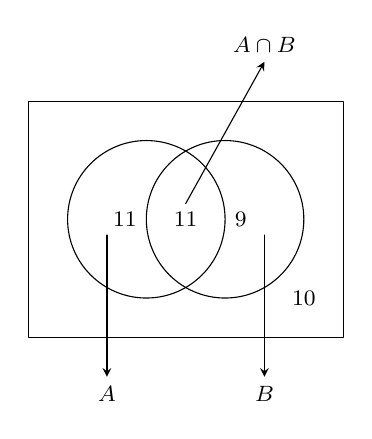
\begin{tikzpicture}[scale=1, font=\footnotesize, line join=round, line cap=round, >=stealth]
		\draw (0,0)--(4,0)--(4,-3)--(0,-3)--cycle;
		\draw (1.5,-1.5) circle (1cm)node[left]{$11$};
		\draw[->][->](1,-1.7)--(1,-3.5)node[below]{$A$};
		\draw (2.5,-1.5) circle (1cm)node[right]{$9$};
		\draw[->](3,-1.7)--(3,-3.5)node[below]{$B$};
		\draw[->](2,-1.3)--(3,0.5)node[above]{$A \cap B$};
		\node at (2,-1.5){$11$};
		\node at (3.5,-2.5){$10$};
	\end{tikzpicture}
\end{center}
\begin{itemchoice}
\itemch Số học sinh chỉ biết chơi bóng rổ là $11$.
\itemch Số học sinh chơi bóng rổ hoặc chơi bóng đá $11+11+9=31$.
\itemch Số học sinh chỉ biết chơi bóng rổ hoặc chỉ biết chơi bóng đá là $11+9=20$.
\itemch Dựa vào sơ đồ Ven, số học sinh của lớp $10$A là $11+11+9+10=41$.
\end{itemchoice}
}
\end{ex}
\begin{ex}%[0D1H4-2]%[Dự án A-Đợt 10 HKII NH24-25-Nguyễn Thanh Phong]
	Cho mệnh đề $P$: \lq\lq Tam giác $ABC$ vuông tại $A$\rq\rq\, và mệnh đề $Q$: \lq\lq Tam giác $ABC$ có $AB^2+AC^2=BC^2$\rq\rq. Xét mệnh đề kéo theo $P \Rightarrow Q$
\choiceTF
{\True Mệnh đề $P \Rightarrow Q$ được phát biểu là: \lq\lq Nếu tam giác $ABC$ vuông tại $A$ thì tam giác $ABC$ có $AB^2+AC^2=BC^2$\rq\rq}
{Trong mệnh đề $P \Rightarrow Q$ thì $P$ là điều kiện cần để có $Q$}
{Mệnh đề đảo $Q \Rightarrow P$ là mệnh đề sai}
{\True Mệnh đề $P \Rightarrow Q$ là mệnh đề đúng}
\loigiai{
\begin{itemchoice}
	\itemch Mệnh đề $P \Rightarrow Q$ được phát biểu là: \lq\lq Nếu tam giác $ABC$ vuông tại $A$ thì tam giác $ABC$ có $AB^2+AC^2=BC^2$\rq\rq.
	\itemch Trong mệnh đề $P \Rightarrow Q$ thì $Q$ là điều kiện cần để có $P$.
	\itemch Theo định lý Pythagores đảo thì mệnh đề đảo $Q \Rightarrow P$ là mệnh đề đúng.
	\itemch Mệnh đề $P \Rightarrow Q$ là mệnh đề đúng.
\end{itemchoice}
}
\end{ex}
\Closesolutionfile{ans}

\begin{center}
	\textbf{PHẦN 3 - Câu trắc nghiệm trả lời ngắn}
\end{center}
\setcounter{ex}{0}

\Opensolutionfile{ans}[ans-OD1-OTC-Deso3-KQ]
\begin{ex}%[0D1V2-1]%[Dự án A-Đợt 10 HKII NH24-25-Nguyễn Thanh Phong]
	Cho hai tập hợp con, khác rỗng của $\mathbb{R}$ là $S=[-8;24)$ và $T=(a-3;20)$. Có tất cả bao nhiêu giá trị nguyên âm của tham số $a$ để $T \subset S$.
\par\shortans[oly]{$5$}
\loigiai{
	Để $T \subset S$ thì $-8\leq a-3<20 \Rightarrow -5\leq a<23$. \\
	Vì ta chỉ nhận giá trị nguyên âm của $a$ nên $a \in \{-5;-4;-3;-2;-1\}$.\\
	Vậy có $5$ giá trị của $a$ để $T \subset S$.
}
\end{ex}
%============Câu 3=======================
\begin{ex}%[0D1V2-1]
	Cho tập hợp $A = \{1; 2; 3; 4; 5; 6\}$. Có bao nhiêu tập con có $3$ phần tử của tập hợp $A$ sao cho tổng các phần tử này là một số lẻ?
\par\shortans[oly]{$10$}
	\loigiai{
Để tổng của ba số nguyên là một số lẻ thì trong ba số chỉ có một số lẻ hoặc cả ba số đều lẻ. \\
Nói cách khác tập con này của $A$ phải có một số lẻ hoặc ba số lẻ.\\
Chỉ có một tập con gồm ba số lẻ của $A$ là $\{1;3;5\}$. \\
Các tập con gồm ba số của $A$ trong đó có một số lẻ là: $\{1;2;4\}$; $\{1;2;6\}$; $\{1;4;6\}$; $\{3;2;4\}$; $\{3;2;6\}$; $\{3;4;6\}$; $\{5;2;4\}$; $\{5;2;6\}$; $\{5;4;6\}$.\\
Vậy có $10$ tập con có $3$ phần tử thoả mãn bài toán.
}
\end{ex}
%============Câu 3=======================
\begin{ex}%[0D1V5-2]%[Dự án A-Đợt 10 HKII NH24-25-Nguyễn Thanh Phong]
	Lớp $10$E có $30$ học sinh giỏi ít nhất một môn Toán, Văn, Anh, trong đó có $6$ học sinh giỏi cả Toán và Văn, $5$ học sinh giỏi cả Văn và Anh, $4$ học sinh giỏi cả Toán và Anh, $3$ học sinh giỏi cả ba môn Toán, Văn, Anh. Tính số học sinh chỉ giỏi đúng một môn Toán hoặc Văn hoặc Anh của lớp $10$E.
\par\shortans[oly]{$21$}
\loigiai{
Ta có:
\begin{itemize}
	\item Số học sinh chỉ giỏi Toán và Văn: $6-3=3$.
	\item Số học sinh chỉ giỏi Văn và Anh: $5-3=2$.
	\item Số học sinh chỉ giỏi Toán và Anh: $4-3=1$.
\end{itemize}
	Ta sẽ minh hoạ bài toán bằng sơ đồ Ven:
	\begin{center}
		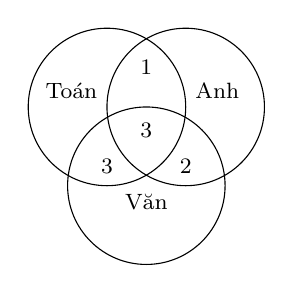
\begin{tikzpicture}[scale=1, font=\footnotesize, line join=round, line cap=round, >=stealth]
			\draw (0,0)circle (1cm)node[left, yshift=.2cm]{Toán};
			\draw (1,0)circle (1cm)node[right, yshift=.2cm]{Anh};
			\draw (0.5,-1)circle (1cm)node[yshift=-.2cm]{Văn};
			\node at (0.5,0.5){$1$};
			\node at (0,-0.75){$3$};
			\node at (1,-0.75){$2$};
			\node at (0.5,-0.3){$3$};
		\end{tikzpicture}
	\end{center}
Từ sơ đồ Ven, số học sinh chỉ giỏi đúng một môn Toán hoặc Văn hoặc Anh là $30-3-2-1-3=21$.
}
\end{ex}
%============Câu 4=======================
\begin{ex}%[0D13V5-1]
	Để thành lập đội tuyển học sinh giỏi khối $10$, nhà trường tổ chức thi chọn các môn Toán, Văn, Anh trên tổng số $111$ học sinh. Kết quả có: $70$ học sinh giỏi Toán, $65$ học sinh giỏi Văn, $62$ học sinh giỏi Anh. Trong đó có $49$ học sinh giỏi cả hai môn Văn và Toán, $32$ học sinh giỏi cả hai môn Toán và Anh, $34$ học sinh giỏi cả hai môn Văn và Anh. Xác định số học sinh giỏi cả ba môn Văn, Toán, Anh. Biết rằng có $6$ học sinh không đạt yêu cầu cả ba môn.
\par\shortans[oly]{$23$}
	\loigiai{Gọi $d$ là số học sinh giỏi cả $3$ môn Toán, Văn, Anh. Ta có: $d=111-6=105$. 
\immini{\begin{itemize}
		\item Số học sinh giỏi Văn và không giỏi Toán là $65-49=16$.
		\item Số học sinh chỉ giỏi Anh và Văn là $34-d$.
		\item Số học sinh chỉ giỏi Anh là $62-32-(34-d)=d-4$.
		\item Số học sinh chỉ giỏi ít nhất $1$ môn là $70+16+d-4=105 \Rightarrow d=23$.\\
		Do đó số học sinh giỏi cả $3$ môn Toán, Văn, Anh là $23$.
	\end{itemize}}
{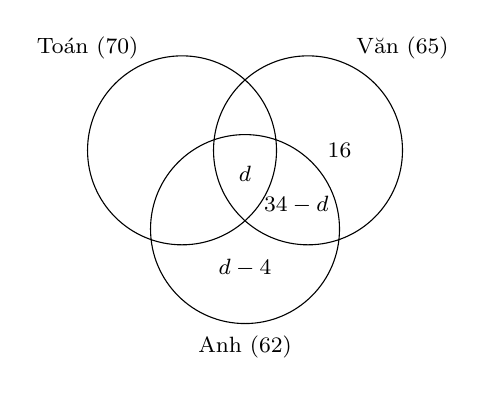
\begin{tikzpicture}[scale=1,font=\footnotesize,line join=round,line cap=round,>=stealth]
    \def\radius{1.2cm}
    \coordinate (C1) at (-0.8, 0.5); 
    \coordinate (C2) at (0.8, 0.5);  
    \coordinate (C3) at (0, -0.5); 
    \draw (C1) circle (\radius);
    \draw (C2) circle (\radius);
    \draw (C3) circle (\radius);
    \node at (-2, 1.8) {Toán $(70)$};
    \node at (2, 1.8) {Văn $(65)$};
    \node at (0, -2) {Anh $(62)$};
    \node at (0, 0.2) {$d$};
	% \node at (-0.5, -0.2) {$32$};
	\node at (0.65, -0.2) {$34-d$};
	\node at (0, -1) {$d-4$};
	\node at (1.2,0.5){$16$};
\end{tikzpicture}}
}
\end{ex}
\Closesolutionfile{ans}


\begin{center}
	\textbf{PHẦN 4 - Phần tự luận}
\end{center}
\setcounter{ex}{0}

\begin{ex}%[0D1H2-1]
Cho tập hợp $A=\{n \in \mathbb{N}^* \mid 3<n^2 < 30\}$. Hỏi tổng tất cả các phần tử của $A$ bằng bao nhiêu?
\loigiai{
Các giá trị $n^2$ thoả mãn $3<n^2 < 30$ là $4$, $9$, $16$, $25$. \\
Vì $n \in \mathbb{N}^*$ nên các giá trị $n$ thoả mãn là $2$; $3$; $4$; $5$.\\
Do đó: $A=\{2;3;4;5\}$.\\
Suy ra tổng tất cả phần tử của $A$ bằng $2+3+4+5=14$.
}
\end{ex}
\begin{ex}%[0D1V3-1]%[Dự án A-Đợt 10 HKII NH24-25-Nguyễn Thanh Phong]%[Unknown]
	Cho hai tập hợp $A=[-4;1]$, $B=(-3;m]$. Biết $B \neq \varnothing$, có bao nhiêu giá trị nguyên của tham số $m$ để $A \cup B = A$.
\loigiai{
	Muốn cho $A \cup B = A$, ta chỉ cần tìm $m$ sao cho $B \subset A$. Do đó $-3 < m \leq 1$. \\
	Vì $m \in \mathbb{Z}$ nên $m \in \{-2;-1;0;1\}$.\\
	Vậy có $4$ giá trị nguyên của $m$ để $A \cup B = A$.
}
\end{ex}
\begin{ex}%[0D1H1-2]
    Cho phương trình $ax^2+bx+c=0$. Xét mệnh đề \lq\lq Nếu $a+b+c=0$, $a \neq 0$ thì phương trình $ax^2+bx+c=0$ có một nghiệm bằng $1$\rq\rq. Mệnh đề này đúng hay sai?
    \loigiai{
Thay $x=1$ vào phương trình $ax^2+bx+c=0$, ta được: $a+b+c=0$. \\
Vậy mệnh đề  \lq\lq Nếu $a+b+c=0$, $a \neq 0$ thì phương trình $ax^2+bx+c=0$ có một nghiệm bằng $1$\rq\rq\, \textbf{đúng}. }
\end{ex}
